% Created 2025-01-16 Thu 18:50
% Intended LaTeX compiler: pdflatex
\documentclass[11pt]{article}
\usepackage[utf8]{inputenc}
\usepackage[T1]{fontenc}
\usepackage{graphicx}
\usepackage{longtable}
\usepackage{wrapfig}
\usepackage{rotating}
\usepackage[normalem]{ulem}
\usepackage{amsmath}
\usepackage{amssymb}
\usepackage{capt-of}
\usepackage{hyperref}
\usepackage{minted}
\usepackage[margin=0.5in]{geometry}
\hypersetup{colorlinks, linkcolor=black}
\usepackage{geometry}
\geometry{top=2cm}
\geometry{bottom=2cm}
\usepackage{fancyhdr}
\pagestyle{fancy}
\fancyhf[L]{Redes de área local}
\fancyhf[R]{Tema 03}
\fancyfoot[R]{ismael.macareno@educa.madrid.org}
\fancyfoot[L]{CC BY-NC-SA 4.0}
\usepackage{parskip}
\usepackage{mdframed}
\usepackage{fancyvrb}
\usepackage{xcolor}
\definecolor{shadecolor}{RGB}{220,220,220}
\newenvironment{shadedcode}{%
\VerbatimEnvironment
\begin{mdframed}[backgroundcolor=shadecolor,linewidth=0pt]}%
{\end{mdframed}}
\usepackage{attachfile2}
\newcommand{\textattachfilecolor}[2]{\textattachfile[color=0 0 0.5]{#1}{\textcolor{blue}{#2}}}
\usepackage[spanish]{babel}
\usepackage{datetime2}
\DTMlangsetup[es-ES]{ord=raise}
\renewcommand{\dateseparator}{/}
\usepackage{titlesec}
\usepackage{afterpage}
\newcommand\blankpage{\null\thispagestyle{empty}\newpage}
\usepackage{colortbl}
\usepackage{pdfpages}
\usepackage{tcolorbox}
\usepackage{listings}
\usepackage[spanish]{babel}
\lstset{
inputencoding=utf8,
extendedchars=true,
literate={ñ}{{\~n}}1 {Ñ}{{\~N}}1 {á}{{\'a}}1 {é}{{\'e}}1 {í}{{\'i}}1 {ó}{{\'o}}1 {ú}{{\'u}}1 {Á}{{\'A}}1 {É}{{\'E}}1 {Í}{{\'I}}1 {Ó}{{\'O}}1 {Ú}{{\'U}}1,
basicstyle=\ttfamily,
breaklines=true,
columns=fullflexible,
keepspaces=true,
language=TeX,
morekeywords={*, -, **, /}
}
\author{Ismael Macareno Chouikh}
\date{\today}
\title{Aspectos Físicos}
\hypersetup{
 pdfauthor={Ismael Macareno Chouikh},
 pdftitle={Aspectos Físicos},
 pdfkeywords={},
 pdfsubject={},
 pdfcreator={Emacs 29.4 (Org mode 9.6.15)}, 
 pdflang={Spanish}}
\begin{document}

\maketitle
\tableofcontents

\blankpage

\section{Conceptos Inciales}
\label{sec:orgc76c7a0}
\subsection{Tipos básicos de medios de red:}
\label{sec:orgfb04d40}
\begin{itemize}
\item \textbf{cable de cobre}
\item \textbf{fibra}
\item \textbf{inalámbrico}
\end{itemize}

\subsection{Tipos de señales / canales de transmisión:}
\label{sec:org7c6f46f}
\begin{itemize}
\item señales analógicas - canales analógicos
\item señales analógicas - canales digitales
\item señales digitales - canales analógicos
\item señales digitales - canales digitales
\end{itemize}

\section{Estándares}
\label{sec:org8467717}
Hay muchas organizaciones involucradas. Las más importantes son:
\begin{itemize}
\item ISO
\item IEEE
\item ANSI
\item entre muchas otras
\end{itemize}

\section{Señalización}
\label{sec:org8a4f6ca}
La capa física debe generar las señales inalámbricas, ópticas o eléctricas que representan el "1" y el "0" en los medios.

\textbf{El método de representación de bits se denomina método de señalización}.

La transmisión de la trama a través de los medios se realiza mediante una \textbf{cadena o stream de bits}.

\subsection{Concepto de tiempo de bit}
\label{sec:org74c7f24}
El tiempo de bit es el tiempo que ocupa el medio la transmisión de un bit.

Para sincronizar los relojes e identificar inicios/finales tramas (información a nivel de enlace), se utilizan combinaciones de bits
preestablecidas (patrones).

\subsection{Señales analógicas}
\label{sec:orgb372a96}
Los bits se representan en el medio al cambiar una o más de las siguientes características de una señal.
\begin{itemize}
\item Amplitud
\item Frecuencia
\item Fase
\end{itemize}

\subsubsection{Ejemplos de modulación de señales}
\label{sec:org605f1fd}
\begin{figure}[htbp]
\centering
\includegraphics[width=.9\linewidth]{../apuntes/img/ejemplo-modulacion-señales.png}
\caption{Macareno, Ismael. (2025). Ejemplo de Modulación de señales [PNG]. Internet}
\end{figure}

\subsubsection{Señales analógicas periódicas (características)}
\label{sec:orge676ca9}
\begin{itemize}
\item \textbf{Amplitud}: medida de la variación máxima del desplazamiento de la onda con respecto a su posición de reposo o equilibrio.
\item \textbf{Ciclo}: oscilación de un punto desde su posición inicial hasta que vuelve a esa posición.
\item \textbf{Periodo (T)}: duración de un ciclo
\item \textbf{Frecuencia (f=1/T)}: es una magnitud que mide el número de repeticiones por unidad de tiempo de cualquier fenómeno o suceso periódico
\item \textbf{Fase}: desplazamiento inicial de la señal
\end{itemize}

\subsubsection{Señales analógicas complejas}
\label{sec:org9b84b05}
\begin{itemize}
\item Una onda compleja se puede ver como la composición de ondas más sencillas con distintas frecuencias.
\item \href{https://es.wikipedia.org/wiki/Transformada\_de\_Fourier}{La transformada de \emph{fourier}} permite encontrar las ondas sencillas que componen un más compleja.
\end{itemize}
\subsection{Señales digitales}
\label{sec:orgb5ac414}
\begin{itemize}
\item Las \textbf{señales digitales} presentan un conjunto de valores discreto, siendo su modo de señalización los diferentes valores que presenta la señal física.
\item La \textbf{tasa de bits} es el número de bits transmitidos por unidad de tiempo.
\item La \textbf{tasa de baudios} es el número de señales por segundo. Un baudio puede estar formada por varios bits.
\end{itemize}
\subsection{Codificación \textbf{digital}}
\label{sec:org2ae968e}
\begin{itemize}
\item \textbf{La codificación es un método que se utiliza para convertir un flujo o conjunto de bits de datos en un código predefinido}
\item La utilización de patrones predecibles permite:
\begin{itemize}
\item Identificar bits de datos y bits de control.
\item Mejora la detección de errores en los medios.
\item Identificar el comienzo y el final de una trama
\end{itemize}
\end{itemize}

\subsubsection{Codificación digital - unipolar, NRZ-L y NRZI)}
\label{sec:orga4319b9}
\begin{itemize}
\item \textbf{Código unipolar}: La amplitud media no es cero. Componente de corriente continua.
\item \textbf{Código NRZ-L}: Sincronización con muchos 0s o 1s seguidos.
\item \textbf{Código NRZI}:
\begin{itemize}
\item 0: la señal con cambia
\item 1: la señal \textbf{se invierte}
\end{itemize}
\end{itemize}

\subsubsection{Codificación digital - RZ}
\label{sec:orge4d9a34}
\textbf{Como NRZL pero a mitad del intervalo se vuelve a cero. Al principio de bit el comportamiento es:}
\begin{itemize}
\item 0: transición de 0 a negativo
\item 1: transición de 0 a positivo
\end{itemize}

\textbf{Requiere 2 transiciones por cada bit.}

\subsubsection{Ejemplo de codificación digital RZ}
\label{sec:org28268b5}
\begin{figure}[htbp]
\centering
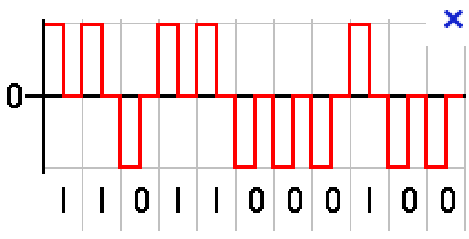
\includegraphics[width=.9\linewidth]{../apuntes/img/ejemplo-codificacion-rz.png}
\caption{Macareno, Ismael. (2025). Ejemplo de codificación digital RZ [PNG]. Internet}
\end{figure}

\subsubsection{Codificación digital - Manchester}
\label{sec:org2145307}
Funciona de la siguiente manera:
\begin{itemize}
\item 0 -> La señal sube de -x a x
\item 1 -> La señal baja de x a -x
\item La transición se realiza a mitad del bit.
\end{itemize}
\subsubsection{Codificación digital - Manchester diferencial}
\label{sec:org32d5829}
Funciona de la siguiente manera:
\begin{itemize}
\item 0 -> Transición al principio
\item 1 -> \textbf{Sin} transición al principio
\item Siempre transición en medio.
\item La transición se realiza a mitad del bit.
\item Permite sincronización entre emisor y receptor
\end{itemize}
\subsubsection{Ejemplo de Manchester diferencial}
\label{sec:org9dc599a}
\begin{figure}[htbp]
\centering
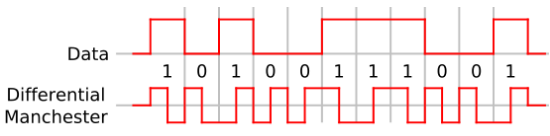
\includegraphics[width=.9\linewidth]{../apuntes/img/ejemplo-codificacion-manchester-diferencial.png}
\caption{Macareno, Ismael. (2025). Ejemplo de codificación en manchester diferencial [PNG]. Internet}
\end{figure}
\subsubsection{Codificación digital - AMI}
\label{sec:orga9a45c4}
Funciona de la siguiente manera:
\begin{itemize}
\item 0 -> 0
\item 1 -> Alterna entre -x y x
\item Problemas para sincronizar muchos 0s seguidos.
\end{itemize}
\subsubsection{Codificación digital - Bipolar con sustitución de 8 ceros (B8ZS)}
\label{sec:org82c9c8f}
Como la AMI, pero cuando aparecen 8 "ceros" consecutivos, se introducen cambios artificiales en el patrón basados en la polaridad del
último bit 'uno' codificado:
\begin{itemize}
\item \textbf{V}: Violación, mantiene la polaridad anterior en la secuencia.
\item \textbf{B}: Transición, invierte la polaridad anterior en la secuencia.
\item Los ocho ceros se sustituyen por la secuencia: 000V B0VB
\end{itemize}
\subsubsection{Ejemplo de B8ZS}
\label{sec:org308470b}
\begin{figure}[htbp]
\centering
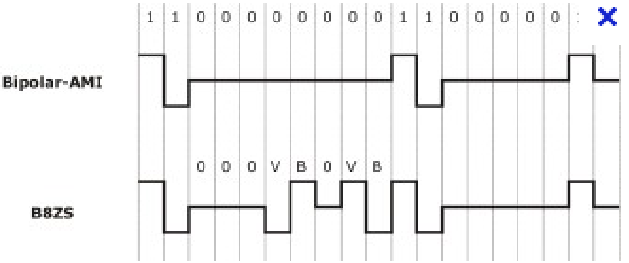
\includegraphics[width=.9\linewidth]{../apuntes/img/ejemplo-codificacion-b8zs.png}
\caption{Macareno, Ismael. (2025). Ejemplo de codificación en B8ZS [PNG]. Internet}
\end{figure}
\subsubsection{Codificación digital - 4B/5B}
\label{sec:orge115dde}
\begin{itemize}
\item En 4B/5B, cada byte que a transmitir se divide en partes de cuatro bits y se codifica según la tabla como valores de cinco bits
\end{itemize}
denominados símbolos.

\begin{itemize}
\item 4B/5B garantiza la aplicación de al menos un cambio de nivel por código para proporcionar sincronización.
\end{itemize}
\subsection{Capacidad del canal para transportar datos}
\label{sec:orgd9bea6d}
\begin{itemize}
\item Se puede medir la transferencia de datos en \textbf{tres formas:}
\begin{itemize}
\item \textbf{Ancho de banda}: capacidad de un medio para transportar datos sin procesar en un tiempo determinado
\item \textbf{Rendimiento}: medida de transferencia de bits a través de los medios durante un período de tiempo determinado.
\item \textbf{Capacidad de transferencia útil}: mide la transferencia efectiva de los datos del usuario entre las entidades de la capa de aplicación
\end{itemize}
\end{itemize}

\subsection{Actividades}
\label{sec:org3e2fa3a}
Codifica los dígitos 1011100010 en:
\begin{itemize}
\item NRZ
\item NRZI
\item AMI
\item Manchester
\item Bipolar con sustitución de 8 ceros
\item 4B/5B
\end{itemize}

\subsection{Señales analógicas en medios digitales}
\label{sec:org9ff43d0}
Los pasos para la conversión de una señal analógica a digital son:
\begin{itemize}
\item muestreo
\item redondeo
\item codificación
\item transmisión
\end{itemize}

La señal se reconstruye en el receptor a partir de información digital.

\begin{itemize}
\item Codificador: transforma de analógico a digital
\item Descodificador: transforma de digital a analógico
\end{itemize}

\subsubsection{Señales analógicas en medios digitales - Muestreo}
\label{sec:orgc3d83c8}
\begin{itemize}
\item se toman medidas de la señal analógica a intervalos regulares
\item a mayor número de muestras por segundo, \textbf{más fiel} es la onda digital resultante
\item es necesario establecer cuántos bits son necesarios para cada medición
\item a mayor número de bits, \textbf{mayor precisión} y \textbf{más fiel} será la onda resultante
\end{itemize}

\subsubsection{Señales analógicas en medios digitales - Redonde y codificación}
\label{sec:org3aec4b8}
\begin{itemize}
\item \textbf{Redondeo:} a mayor número de muestras obtenidas, la señal digital reflejará con mayor precisión la señal analógica que reproduce. Aquellos valores de la señal analógica que no se
consideran en la digital, deberán ser redondeados al valor digital mas próximo.
\item \textbf{Codificación:} en última instancia, la transmisión por el medio será digital binaria
\item \textbf{Envío por canal digital:} para el envío final, se podrá utilizar cualquiera de los modelos de codificación digital vistos anteriormente
\end{itemize}

\section{Multiplexación}
\label{sec:org17e3b12}
\subsection{¿De qué trata?}
\label{sec:org2cb277c}
\textbf{técnica que permite compartir el medio entre diferentes usuarios para obtener el mejor aprovechamiento de su ancho de banda}

\subsection{Multiplexación por división de \textbf{frecuencia}}
\label{sec:orge4fa496}
\begin{itemize}
\item Se asigna una banda de frecuencias concreta a cada canal lógico.
\end{itemize}
\subsection{Multiplexación por división en \textbf{tiempo}}
\label{sec:org6ecdb90}
\begin{itemize}
\item Se divide el tiempo en ranuras.
\item Cada canal obtiene determinadas ranuras de tiempo.
\end{itemize}

\section{Sincronización}
\label{sec:orga2c4e2d}
Proceso mediante el cual el equipo receptor, conoce los momentos exactos en que debe medir la magnitud de la señal para identificar la información recibida

\subsection{Multiplexación - Transmisión \textbf{asíncrona}}
\label{sec:org171908d}
\begin{itemize}
\item Las señales que permiten marcar los tiempos están incluidas en el mensaje transmitido
\item En el mensaje hay algunos bits que sirven para sincronizar emisor y receptor.
\item Los datos se transmiten enviándolos carácter a carácter, donde cada carácter tiene una longitud de 5 a 8 bits
\item El receptor tiene la oportunidad de resincronizarse al principio de cada carácter.
\item Requiere de 2 o 3 bits suplementarios por cada carácter
\item Sencilla y no costosa
\end{itemize}

\subsection{Multiplexación - Transmisión \textbf{síncrona}}
\label{sec:org22eeccb}
\begin{itemize}
\item Los bits se envían a una velocidad constante sin diferenciar los caracteres que componen.
\item El emisor y el receptor utilizan relojes a la misma frecuencia.
\item El comienzo y el final de cada bloque de datos se identifican con patrones de bits conocidos en ambos lados de la comunicación.
\item Permite velocidades de transmisión mayores
\end{itemize}


\section{Modos de transmisión}
\label{sec:orgc46f14e}
\subsection{Transmisión \textbf{serie}}
\label{sec:org97d54a5}
\textbf{Todas las señales se transmiten por una única línea de datos secuencialmente}
\subsection{Transmisión \textbf{paralelo}}
\label{sec:orgb321ecb}
\textbf{Se transmiten simultáneamente un grupo de bits, uno por cada línea del mismo canal.}
\section{Perturbaciones en la transmisión}
\label{sec:org2589a39}
\begin{itemize}
\item En una transmisión, la señal recibida puede ser distinta de la emitida por culpa de perturbaciones:
\end{itemize}
\subsection{Atenuación}
\label{sec:org4a8944f}
\begin{itemize}
\item Debilita la señal
\item La amplitud disminuye
\end{itemize}
\subsection{Distorsión}
\label{sec:org9bb14b8}
\begin{itemize}
\item Deformación de la señal por el hecho de que la velocidad de propagación de la señal en el medio varía con las características de la señal misma
\end{itemize}
\subsection{Interferencia}
\label{sec:org8b1976d}
\begin{itemize}
\item Suma a la señal que se transmite de otra señal conocida y no deseada.
\end{itemize}
\subsection{Ruido}
\label{sec:org7cdf7c7}
\begin{itemize}
\item Es la suma de múltiples interferencias, posiblemente de origen desconocido y de naturaleza aleatoria.
\item El ruido se puede aislar solo en ciertos casos.
\end{itemize}
\subsection{Diafonía}
\label{sec:org2968281}
\begin{itemize}
\item Parte de las señales presentes en uno de ellos, considerado perturbador, aparece en el otro, considerado perturbado.
\item Ejemplo: escuchar a otra conversación por teléfono.
\end{itemize}
\end{document}
